\section{System Architecture}
\label{sec:chap06:systemDesign}
In a standard DASH based streaming environment, a content server keeps the entire video in multiple quality levels. The video files are divided into many small segments, and every segment is encoded with multiple supported quality levels. Most of the time, the duration and start time of all the segments across different qualities are the same. In the case of live streaming, the content server populates the segments on the fly as the stream progresses. As we mentioned earlier, the captured video is processed at the content server in chunks of predefined playback duration. The entire video chunk is divided into segments of small length, and each segment is encoded into multiple quality levels. Depending on the network condition, a DASH-based streaming player downloads the available segments of the desired quality level.
%\begin{figure}[!ht]
%    \centering
%    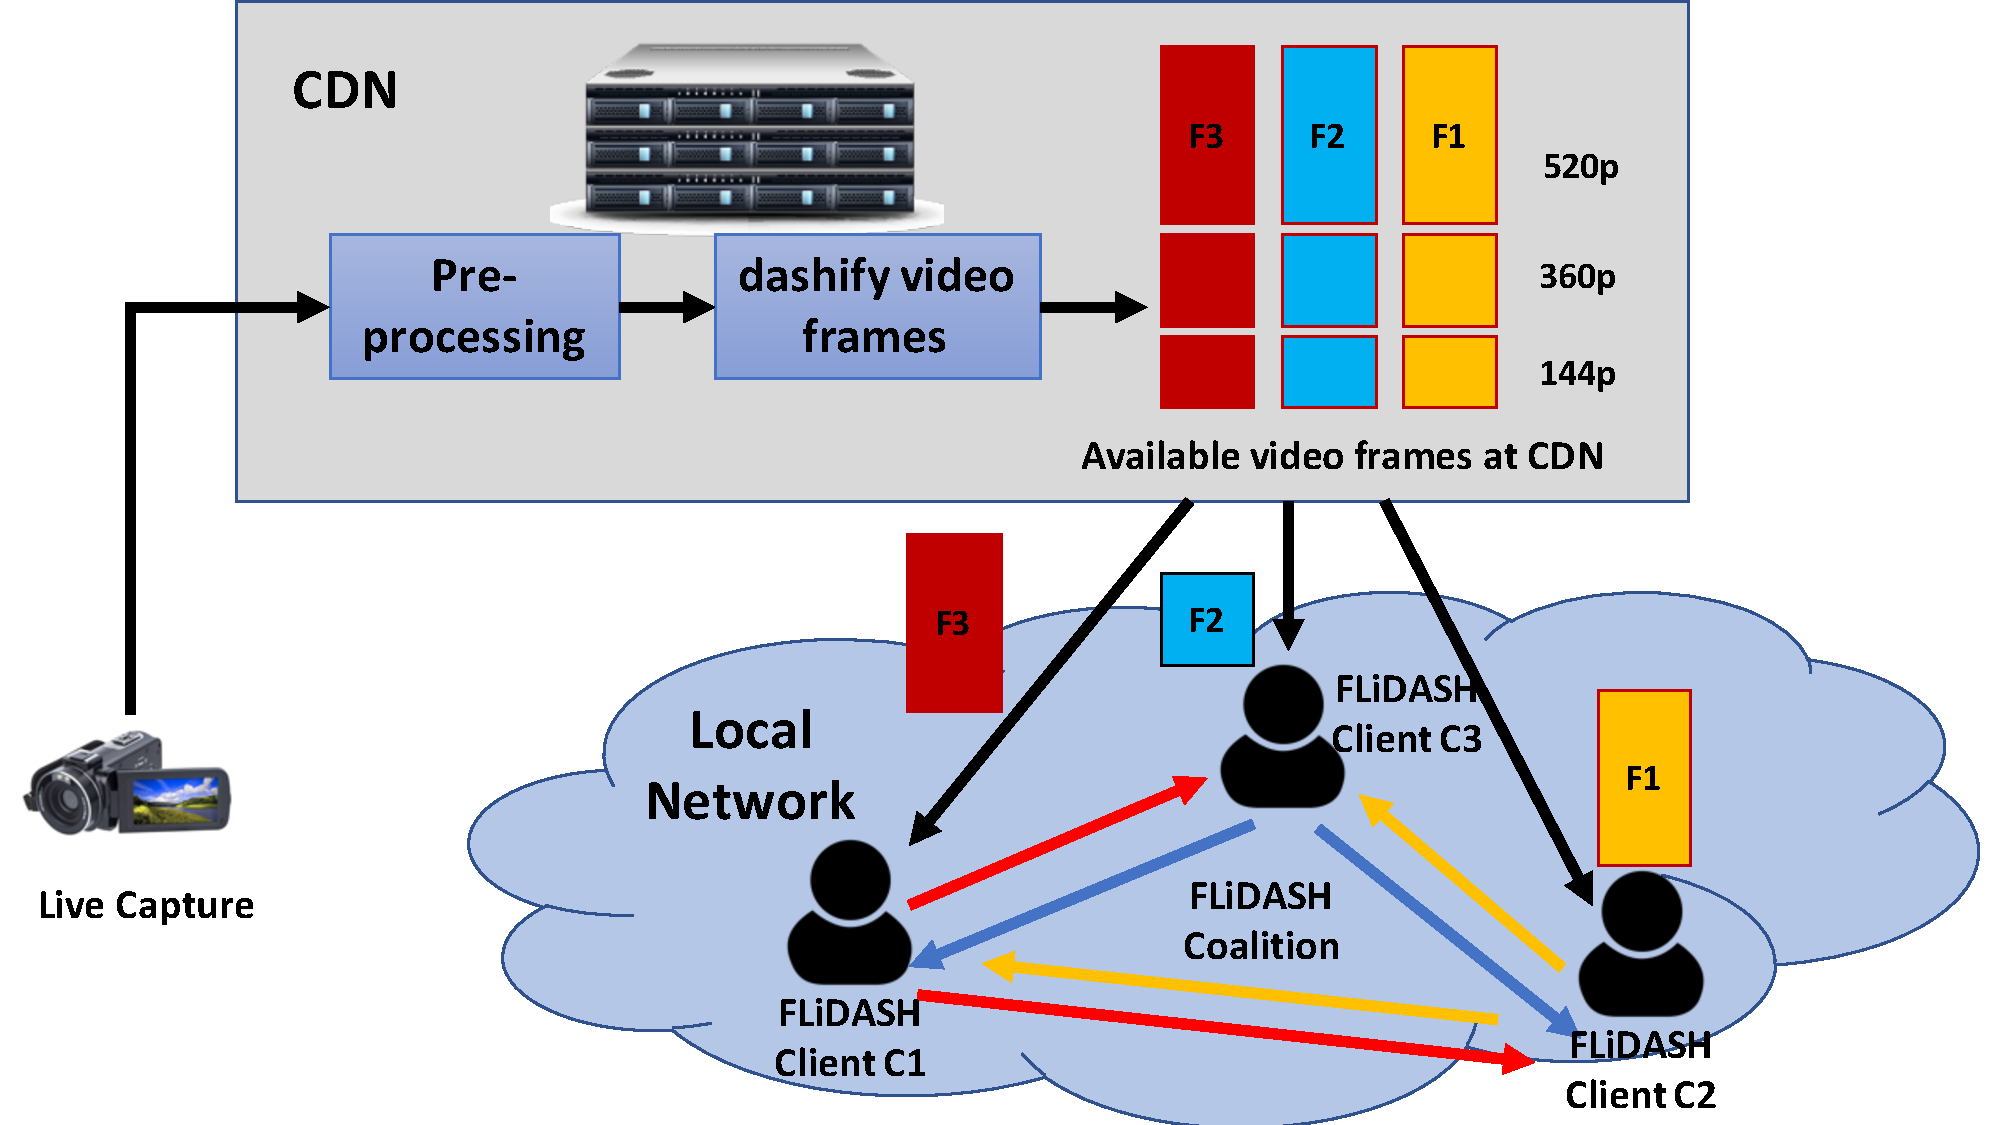
\includegraphics[width=\linewidth]{img/flsd.pdf}
%    \caption{Overview of \our: The clients under a local network creates a coalition, every member of the coalition shares the total download load.}
%    \label{fig:flsd}
%\end{figure}
%\fig\ref{fig:flsd} gives a broad overview of \our -- 

In contrast to the DASH client-server architecture, {\our} forms multiple coalitions of players who want to watch a live video, although the network quality of individual players in the coalition can fluctuate over time. %\fig\ref{fig:flsd} shows the overview of the {\our} functionality. 
The live captures are processed at the content delivery network (CDN) server to `dashify' the videos, which converts each video segment into different supported quality levels. Any existing approaches for live video dashification~\cite{wei2014low,pires2014dash} can be used for this purpose; {\our} does not require any changes in the CDN or the working of the streaming server. The streaming clients dynamically form coalitions based on their experience of the network bandwidth as per the spatial proximity (for example, the streaming clients under a same organizational network). Once the coalition is formed, it employs a scheduling policy to download the video segments by different players in the coalition at different times and share them over the coalition. The advantage of this scheme is that a player already knows from whom it is supposed to get the next video segment, based on the scheduling algorithm. {\our} ensures a fair load among the streaming clients in terms of getting data directly from the CDN server.
{\our} has three components as shown in \fig\ref{fig:chap06:playerdiagram}.

\noindent (1) {\bf Streaming Server:} The streaming server is a content delivery  network (CDN) server which encodes the live videos and hosts the video segments. We consider a scenario of a slightly delayed broadcast of the live streaming contents~\cite{huysegems2015http}, where a playout delay (in the order of a few seconds) is introduced between the content recording and the content broadcast, within which the content server can process the recorded video segments to encode them in multiple DASH-supported bitrates. As a consequence, at any instance of time, a few number of DASH-encoded video segments are available at the content server for downloading them in parallel. It can be noted that such a playout delay is common in many commercial live streaming systems~\cite{zinner2017comparison}. 
\begin{figure}[!ht]
	\centering
	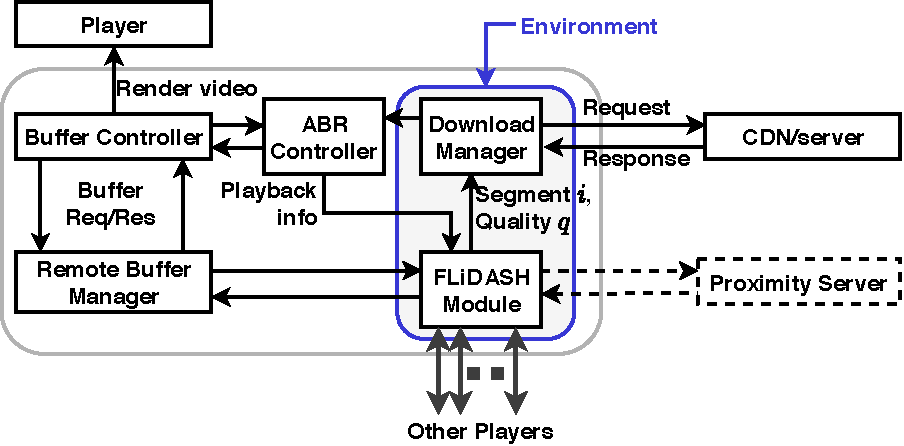
\includegraphics[width=0.8\linewidth]{img/PlayerDiagram}
	\caption{\label{fig:chap06:playerdiagram} Architectural Components for \our}
\end{figure}

\noindent (2) {\bf Proximity Server:} It keeps the locality information about the video players who stream the same live video content. A streaming server or a player can act as the Proximity server. However, if the network have an ALTO service, the coalition formation becomes easier~\cite{alimi2014application}. ALTO mainly provides two basic pieces of information -- a cost map and a network map. These two pieces of information help the player to understand the distance and delay from another player. Without the ALTO service, FLiDASH players have to ping or traceroute to understand the distance and delay, which is comparatively more expensive.
%\sout{An ALTO server~\cite{alimi2014application} or even the streaming server can work as a proximity server.}
%It can be noted that any existing video streaming client (or even the streaming server) can work as a proximity server as well. Further, this proximity server is different from the P2P controller as used in existing systems~\cite{detti2016tracker,khalid2019sdn,payberah2012clive,wang2014migration}, as it does not need any computation or processing capability, it just keeps the players' information which all the clients in a coalition can access. 

\noindent (3) {\bf Player:} A video player renders the video at the end-user side as well as creates and maintains the coalition. Each player consists of three modules -- i) \textit{Playback}, ii) \textit{Environment}, and iii) \textit{Adaptive Bit Rate} (ABR). A {\it Playback} module keeps track of the playback buffer and the playback time. The {\it Environment} module forms a coalition with the nearby players and shares segments among other players in the coalition, following a distributed policy enforcement principle.
%Each Player has limited buffer capacity; it cannot store the next segment unless it has enough space in the buffer. However, segments can be pushed to the playback buffer without maintaining the order. {\our} uses an explicit buffer management strategy, as discussed later, to handle the ordering of video frames. 
Every time it receives a segment, the playback module asks the {\it ABR} module for the next quality level and the sleep-time before it can start downloading. The sleep-time dictates the frequency of attempting a direct download from the CDN. 
%The {\it ABR} module calculates the next quality level and the sleep-time. We can use any existing ABR algorithm for this module when a streaming client has not joined in a coalition; in our implementation, we can choose from Rate-based (standard DASH algorithm), Buffer-based~\cite{buffer-based-sigcomm-2014}, BOLA~\cite{bola1-infocom-2016}, MPC~\cite{yin2015control} and Pensieve~\cite{Pensieve} as the standalone rate adaptation algorithms. However, these existing approaches for adaptive streaming consider the states of a single-player only and therefore fail to capture the collective states of a coalition. {\our} uses a novel mechanism for the bitrate selection depending on the collective states of all the members of the coalition.

%The {\it ABR} module calculates the sleep-time in such way so that the {\it Environment} module, as described next, completes downloading the next segment exactly when the player frees up enough space for that segment. The {\it Environment} module is responsible for downloading the segments.
%It predicts the download time based on the network condition and generates the next event based on the download time.




%\section{Design and Implementation}
%\label{sec:groupDesign}
%In this section, we describe the detailed system design and implementation aspects of \our.

\section{Streaming Coalition Formation}
%{\our} forms coalitions among \textit{``similar"} players so that they can divide and share the DASH video segments among themselves to collectively download the video content and render them with playback synchronization. We define similarity based on the average network condition faced by a player, although the instantaneous network quality may change over time. 
To form a coalition, {\our} first uses the expected playback quality for a player based on its view-port size and resolution (for example, playing a video on a laptop requires higher quality level than playing it over a smartphone, to ensure similar QoE for the user), along with the average network bandwidth. To estimate the average network bandwidth, a player $P_i$ waits for some time to download $\mathcal{T}$ number of video segments directly from the streaming server with a server-client based ABR algorithm~\cite{bola2-acm-mmsys2018,yin2015control,mao2017neural} and measures the throughput $\tau_i$ based on the amount of data downloaded.
%Once $\tau_i$ is determined, player $P_i$ set the target quality $\mathcal{Q}_{p_i}$ based on any existing ABR algorithm.
Let $\mathcal{Q}_G$ and $\mathcal{Q}_{P_i}$ be the average playback quality of a coalition $G_p$ and a player $P_i$. The player $P_i$ tries to find a coalition $G_p$ in the vicinity (based on the information received from the \textit{Proximity Server}) such that (a) $P_i$ is within the same network of the existing players in $G_p$ (all the players are behind a common core network gateway), (b) $\mathcal{Q}_G \approx \mathcal{Q}_{P_i}$, (c) $\forall_{P_k \in G_p} delay(P_i, P_k) < t_d$ (using the cost map and network map from the ALTO server) where $t_d$ is a threshold on the permissible delay between two coalition members\footnote{In all of our experiments, we used $t_d=$8 ms, which has been decided empirically based on the impact of this parameter on the performance of the system.}, and (d) the current playback time of the player $P_i$ has a maximum one segment delay from the current playback time of the coalition (this condition ensures playback synchronization during coalition formation). If no such coalition exists in the vicinity, the player continues as a standalone player until another player joins to form a coalition. 
%The coalition information is registered on the proximity server.
%
%\begin{algorithm}[h]
%	Start\;
%	$\tau_i = 0$\;
%	$z = 0$\;
%	\While{True}{
%		WaitForNextRequest()\;
%		\eIf{Group formed?}{
%			waitToRecvSegFromGroup()\;
%			sendSegmentToPlayer()\;
%		}{
%			downloadBasic()\;
%			sendSegmentToPlayer()\;
%			$z = z + 1$\;
%			\If{$z \ge \mathcal{T}$}{
%				$\tau_i \leftarrow$ measureThroughput()\;
%				formGroup($\tau_i$)\;
%			}
%		}
%	}
%	\caption{Group formation algorithm}
%	\label{algo:groupFormation}
%\end{algorithm}
%\notesc{segment and chunk -- both the terms has been used -- use only ``segment".}

%In \our, we expect that the latency between two coalition members is lesser than the latency between the streaming server and the client. We can find this type of scenario when multiple users share a common Internet backbone, or in case of Internet-on-cable where ISP connects multiple customers over a LAN. However, the Internet bandwidth of individuals can be different. With these preconditions, we keep target video bitrate $\mathcal{Q}_g$ around $\min(2\times\tau_i, V_i)$, where $V_i$ is the maximum quality supported by the viewport.
%It will give enough time to download a video segment with higher bitrate than its bandwidth.

After the coalition formation phase, we need to distribute the responsibility of segment downloading among the coalition members. Here each player collaboratively tries to increase the overall QoE of the coalition. However, it is crucial that the players in a coalition stay in playback sync, i.e. every player in a coalition needs to play approximately the same video segment. Every player needs to go through a synchronization (discussed later) step during the coalition formation. In a steady state, every player stays in sync as all of them gets a video segment almost at the same time.

\section{Segment Download and Distribution}
The Internet bandwidth between a player and the content server may change over time, and this change may be different for different {\our} players. Therefore, the coalition needs to take two collective decisions -- (i) which player would download the next video segment, and (ii) what would be the download quality of the next video segment depending on the collective QoE of the coalition. {\our} selects an owner for every video segment $s_i$ ($\mathcal{O}_{s_i}$), which download the video segment, as well as takes two decisions -- (a) the bitrate of the downloaded video segment $s_i$, and (b) the owner of the next video segment $s_{i+1}$ ($\mathcal{O}_{s_{i+1}}$). Once $\mathcal{O}_{s_i}$ elects $\mathcal{O}_{s_{i+1}}$, this information is broadcast among the coalition members through gossip protocol. The details follow. 
%Although a coalition is formed based on the average network bandwidth of a player, the instantaneous network quality over time may change drastically from the initial video start-up phase. We set our goal in a way so that a player with a better network quality overtime should not suffer due to a player which experiences low network quality during the playback after joining a coalition. Also, we do not want a player to be a free rider; every player has to contribute to the coalition.
%Therefore, we define a fairness metric which is a function of the total download time to download the segment directly from the streaming server and the part of it that individual players download.
%\notesc{The fairness need to be pointed out -- may not be here, but at the proper place, how this is ensured. This function has never been mentioned later. At what stage this is handled, and how.} \noteam{I am trying to find out}
%So, in \our, a coalition needs to take two decisions collectively -- i) which player would download the next DASH video segment, and ii) what would be the quality for the next video segment based on collective QoE of the coalition. We use an approach to select an owner for every video segment such the the responsibility of the owner is to download the video segment at a computed bitrate and share the segment among other members of the coalition. In our algorithm, the owner of each segment takes two decisions -- i) the bitrate for the current video segment and ii) the owner of the next video segment. It can be noted that the owner of the current video segment can also elect itself as the owner of the next video segment; in that case it downloads two video segments consecutively, as we discussed later. The owner selection should be made as soon as possible to maximize the parallel downloads of video segments; however, a owner can decide the quality level of a video segment just before sending the request to the server.
%We call this leadership process.
%\begin{algorithm}[!ht]
%	%\scriptsize
%    %\small
%	\DontPrintSemicolon
%	\caption{\label{algo:leadership}$OwnerShip()$ -- Schedule collaborative segment downloads by coalition members}
%	\KwIn{$P_i, S_i$}
%
%	\While{$isNotAvailable(S_i)$ }{
%		$sleep(\delta)$ \hspace{1mm} //\texttt{Wait until the segment $S_i$ is available}\;
%	}
%
%	\While{$noBufferAvailable(P_i)$}{
%		$sleep(\delta)$ \hspace{1mm} //\texttt{Wait until the buffer is available} \;
%	}
%
%	$P_{i+1} \leftarrow findNextLeader()$\;
%	$LeaderShip(P_{i+1}, S_{i+1})$ \hspace{1mm} //\texttt{Broadcast} \;
%	$\mathcal{Q}_i \leftarrow findCurrentQuality()$\;
%	$DownloadAndDistribute(P_i, S_i, \mathcal{Q}_i)$\;
%\end{algorithm}
%\algo\ref{algo:leadership} summarizes the process for playback scheduling in a coalition.
%Here the subroutine $OwnerShip(P_i, S_i)$ informs every players (through gossiping) in the coalition that player $P_i$ is the owner for the segment $S_i$. This procedure runs asynchronously whenever a player is selected as the owner of a segment and ensures that only one player downloads a segment and other players retrieve the segment from the owner. Every player waits for a time duration (sleep time) to ensure the availability of a live video segment in the streaming server as well as the availability of the player buffer to store the current segment before it starts downloading.
\subsection{Owner Selection for the Next Segment\label{sec:nextLeadSelect}} In {\our}, the owner of each segment is selected based on the following objectives -- (i) maximize parallel downloads of video segments from the content server, (ii) max-min fair download load allocation among the coalition members, (iii) maximize the playback bitrate of the coalition, (iv) maintain playback synchronization among coalition members. 

As we mentioned earlier that the playout delay at the content server ensures the availability of a few number of video segments encoded in different supported bitrates, the coalition members download them in parallel. The owner selection mechanism distributes the segments among the coalition members based on their instantaneous Internet bandwidth. For example, if a player $P_1$ has twice the Internet bandwidth than another player $P_2$, then player $P_2$ should download one video segment from the CDN, while the player $P_2$ should download two video segments of the same quality level within the same instance of time. Therefore, a total of three video segments can be downloaded collectively by the two players in parallel; they can share the remaining segments with each other for the video playback.    

%As different players experience different network quality over time, we need to schedule segment downloads in such a way so that every player gets enough time to download the video segment without compromising the quality; hence,  a player with a poor network quality should get more time to download a segment than a player with a better network quality. For example, if a player $P_1$ has twice the network bandwidth than another player $P_2$, then player $P_2$ should download one video segment from the streaming server, while the player $P_2$ should download two video segments of the same quality level within the same instance of time. Therefore, a total of three video segments can be downloaded collectively by the two players in parallel; they can share the remaining segments with each other for the video playback. The ABR algorithm takes care of deciding the optimal quality level based on the aggregated bandwidth experienced by all the members of the coalition.

%\notesc{I am not sure, does your approach ensure that players can download video segments in parallel?} \noteam{A player cannot download two segments parallelly.}
%The size of the playback buffer is another important metric for the selection of the owner to download the next video segment. Every browser-based player has a limited buffer \cite{sengupta2018hotdash}.
%To overcome the limited buffer issue, we use a remote buffer management scheme which allows us to extend the playback buffer beyond its limit, as we discuss in the next subsection. 
Based on the above principal, $\mathcal{O}_{s_{i}}$ uses \eqn\ref{eqn:chap06:nextLeader} to find $\mathcal{O}_{s_{i+1}}$. Here, $\mathcal{I}_x$ is the duration (idle time) from the last download for $\mathcal{O}_{s_{x}}$. $\mathcal{D}{q_x}$ and $\mathcal{D}{l_x}$ are the download queue length (i.e. number of pending segments to be download) at $\mathcal{O}_{s_{x}}$ and the download status\footnote{If the segment length is $m$ bytes, and $n$ bytes has been downloaded as of now, them  $\mathcal{D}{l_x} = \frac{m-n}{m}$ } of the ongoing download, respectively. $\mathcal{I}_{max}$ and $\mathcal{D}q_{max}$ are maximum possible idle time (which is $groupsize\times segment\_duration$) and maximum possible download queue length (same as play buffer length in term of number of segments).
\begin{align}
\label{eqn:chap06:nextLeader}
\mathcal{O}_{s_{x}} &= \underset{x \in G_p}{\mathrm{argmax}} \left( {\mathcal{I}_x}/{\mathcal{I}_{max}} - {\mathcal{D}{q_x}}/{\mathcal{D}q_{max}} - \mathcal{D}{l_x} - \mathcal{M}_x \right)
%f(x) &=
\end{align}
\eqn\ref{eqn:chap06:nextLeader} selects $\mathcal{O}_{s_{x}}$ who is idle for the longest time (by looking at the $\mathcal{I}_x$) among all the players in the coalition. In case all the players are busy downloading video segments, the equation considers the download load ($\mathcal{D}{q_x}$ and $\mathcal{D}{l_x}$) on every player. To make sure that the furthest segment should be allocated to the slowest player (which is important for playback synchronization), we calculate the \textbf{deadline miss penalty} $\mathcal{M}_x$. Every direct download from the CDN server is associated with a deadline. $\mathcal{M}_x$ is a function that returns zero if the deadline has not been missed by player $x$ during the last download operation; otherwise, it calculates a penalty based on the deadline miss duration and the current time. So, the player with the lowest load and the highest bandwidth is selected as the owner of the next segment.

\subsection{Forceful Self-download} {\our} expects that corresponding owners would be able to download the segment before its playback time; otherwise, the coalition players may experience a stall time to rebuffer the video, which severely degrades their QoE. However, we cannot avoid this situation completely as the bitrate selection decision is based on the observation of the historical throughput and the instantaneous measure of the available bandwidth; whereas the owner may experience a sudden bandwidth drop during the actual download of the target segment. To avoid this situation, we put a deadline for each segment. If a owner fails to download the segment before the deadline (other players in the coalition fail to fetch the segment from the download buffer of the owner), other players in the coalition who are free at that time (within the sleep-time duration) trigger a forceful self-download of the segment at a low quality, to avoid rebuffering due to a loss in playback synchronization.
\begin{algorithm}[!ht]
	%\scriptsize
    %\scriptsize
	\DontPrintSemicolon
	\If{$d_t \le 0$}{
		$m^*_{n} = 0$\;
		{\bf Return}
	}
	$m^*_{n} \leftarrow m^*_{n-1}$ \; \label{algo:chap06:quality:line:mstar}
	$\varTheta \leftarrow \min(\varTheta_w, \varTheta_{last}, \varTheta_h)$ \; \label{algo:chap06:quality:line:theta}
	%	$t_l \leftarrow d_t - \sum_{x \in \mathcal{D}_{q}} Cl_{x,m^*_{x}} / \varTheta$\;
	$m^\prime \leftarrow \underset{m \in \mathcal{Q}}{\mathrm{argmin}} \{\left| d_t - \frac{Cl_{n,m}}{\varTheta}\right| \} $\; \label{algo:chap06:quality:line:mprime}
	\eIf{$m^\prime > m^*_{n}$}{
		\If{$m^*_{n-1} = m^*_{n-2}$ {\bf and} $m^*_{n-2} = m^*_{n-3}$}{
			$m^*_{n} \leftarrow m^*_{n-1}+1$ \label{algo:chap06:quality:line:increment}
		}
	}{
		$m^*_{n} = \lceil\frac{m^\prime + m^*_{n}}{2} \rceil$
	}
	\caption{\label{algo:chap06:quality}findCurrentQuality()}
\end{algorithm}
\section{Bitrate Selection}
{\our} uses a dynamic tuning approach for bitrate selection based on collective influence of the coalition members. To select the bitrate for segment $s_i$, we use \algo\ref{algo:chap06:quality}. This algorithm executes just before a player starts downloading a segment. In the algorithm, $\varTheta$ is the measured throughput share of the current player in comparison to the total bandwidth available for the coalition. The measured throughput has three components -- the weighted throughput ($\varTheta_w$) which changes its value slowly over the time,  $\varTheta_{last}$ which is the throughput measured during the last finished download by the current player, and $\varTheta_h$ is the harmonic mean of the throughput observed till now. The weighted throughput $\varTheta_{w}$ is measured as $\varTheta_{w_i} = 0.8 \times \varTheta_{w_{i-1}} + 0.2 \times \varTheta_{last}$. We use $\varTheta$ as the minimum of $\varTheta_w$, $\varTheta_{last}$, and $\varTheta_h$, because it is the worst throughput the player observed till now. As we use $\varTheta$ to predict the time require to download a segment, it gives us a worst time bound. $d_t$ is the time left to download the segment $s_i$ so that no player in the coalition stalls. $Cl_{i,j}$ is the content length of the $i^{th}$ segment at the quality level $j$. $m^*_i$ is the selected quality level for the $i^{th}$ segment. \algo\ref{algo:chap06:quality} allows the coalition to increase the video quality when there is a steady network. So, we do not put any restriction in the upper limit of the bitrate even though it involves slight risk of additional stalls and bitrate fluctuations. We analyze the individual QoE parameters in the evaluation, as discussed in the next section.